\section*{4. Ecuaciones diferenciales ordinarias}

El movimiento de un péndulo que se balancea asumiendo ciertas simplificaciones es descrito por una ecuación diferencial de segundo orden:

\begin{equation*}
    \frac{d^2\theta}{d t^2} +\frac{g}{L}sin\theta=0.
\end{equation*}

Donde L es el ángulo del péndulo, $g\approx9.81 m/s^2$ es la constante gravitacional de la tierra y $\theta$ es el ángulo que el péndulo hace con la vertical. Además, se especifica que el movimiento inicia en  $\theta(t_0)=\theta_0$ y su velocidad en dicho punto es $\theta'(t_0)=\theta'_0$; estas especificaciones se llaman \textbf{condiciones iniciales} y el problema se conoce como \textbf{problema con condiciones iniciales o valores iniciales}. Para valores pequeños de $\theta$ la aproximación $\theta\approx sin\theta$ puede ser utilizada para simplificar el problema a un problema lineal con condiciones iniciales:

\begin{equation*}
    \frac{d^2\theta}{d t^2} +\frac{g}{L}\theta=0, \ \ \theta(t_0)=\theta_0, \ \ \theta'(t_0)=\theta'_0.
\end{equation*}

Este problema ahora puede ser resuelto con las técnicas tradicionales de ecuaciones diferenciales.

\subsection*{4.1 Método de Euler}

El método de Euler es la técnica de aproximación más sencilla para resolver los problemas con condiciones iniciales. El objetivo del método de Euler es obtener aproximaciones al problema con valores iniciales.

\begin{equation*}
    \frac{dy}{dt}=f(t,y), \ \ a\leq t\leq b, \ \ y(a)=\alpha.
\end{equation*}

Sin embargo, este método no obtendrá una aproximación a $y(t)$ sino una aproximación a $y$ en varios valores -llamados \textbf{puntos malla}- en el intervalo $[a,b]$ y una vez encontrada la solución aproximada en dichos puntos las siguientes soluciones aproximadas de los otros puntos serán calculadas mediante interpolación.

Primero se realiza la estipulación de que los puntos malla están uniformemente distribuidos en el intervalo $[a,b]$. Esta condición se asegura eligiendo un número entero positivo N y seleccionando los puntos de malla de la siguiente manera:

\begin{equation*}
    t_i=a+ih, \ \ \ \ con \ \ i=0,1,2, \dotsc, N.
\end{equation*}

La distancia $h$ es comúnmente llamada \textbf{tamaño de paso} y se calcula mediante $h=(b-a)/N=t_{i+1}-t_i$. 

Ahora se usará el teorema de Taylor para derivar el método de Euler. Suponga que $y(t)$, la única solución a la ecuación $\frac{dy}{dt}=f(t,y)$, tiene dos derivadas continuas es el intervalo $[a,b]$ entonces para cada $i=0,1,2, \dotsc, N$, 

\begin{equation*}
    y(t_{i+1})=y(t_i)+(t_{i+1}-t_i)+\frac{(t_{i+1}-t_i)^2}{2}y''(\xi_i),
\end{equation*}

para un número $\xi_i$ en $(t_i,t_{i+1})$. Pero como $h=t_{i+1}-t_i$ se obtiene: 

\begin{equation*}
    y(t_{i+1})=y(t_i)+h y'(t_i)+\frac{h^2}{2}y''(\xi_i),
\end{equation*}

pero como $y(t)$ satisface la ecuación diferencial original,

\begin{equation*}
    y(t_{i+1})=y(t_i)+h f(t_i,y(t_i))+\frac{h^2}{2}y''(\xi_i).
\end{equation*}

El método de Euler considera $wi\approx y(t_i)$ para cada $i=0,1,2, \dotsc, N$, por eliminación del término restante. Así, el método de Euler es: 

\begin{equation*}
\begin{split}
    w_0&=\alpha \\
    w_{i+1}&=w_i+hf(t_i,w_i), \ \ para \ cada \ i=0,1,2, \dotsc, N-1.
\end{split}
\end{equation*}

\subsubsection*{Ejemplo}

Utilice el método de Euler para aproximar la solución a

\begin{equation*}
    y'=y-t^2+1, \ \ 0\leq t\leq 2, \ \ y(0)=0.5.
\end{equation*}

en $t=2$. Simplemente se ilustrará los pasos de la técnica cuando se tiene $h=0.5$. 

Para este problema $f(t,y)=y-t^2+1$, entonces

\begin{equation*}
\begin{split}
    w_0&=y(0)=0.5; \\
    w_1&=w_0+0.5(w_0-(0.0)^2+1)=0.5+0.5(1.5)=1.25; \\
    w_2&=w_1+0.5(w_1-(0.5)^2+1)=1.25+0.5(2.0)=2.25; \\
    w_3&=w_2+0.5(w_2-(1.0)^2+1)=2.25+0.5(2.25)=3.375;
\end{split}
\end{equation*}

Entonces

\begin{equation*}
    y(2)\approx w_4=w_3+0.5(w_3-(1.5)^2+1)=3.375+0.5(2.125)=4.4375.
\end{equation*}


\begin{tcolorbox}[colback=blue!15!]
\subsubsection*{Método de Euler}
Para aproximar la solución del problema con valores iniciales

\begin{equation*}
    y'=f(t,y), \ \  a\leq t\leq b, \ \ y(a)=\alpha,
\end{equation*}

en un intervalo [a,b] dividido en (N+1) del mismo tamaño:
\\ \\
ENTRADA Puntos extremos a,b; entero N; condición inicial $\alpha$.

SALIDA Aproximación $w$ a $y$ en $(N+1)$ valores de $t$.
\\ \\
PASO 1 Asigna h=(b-a)/N;

\ \ \ \ \ \ \ \ t=a;

\ \ \ \ \ \ \ \ $w=\alpha$;

\ \ \ \ \  SALIDA (t,w).

PASO 2 Para $i=1,2,\dotsc, N$ ejecuta los pasos 3 y 4.

\ \ \ \  PASO 3 Asigna $w=w+hf(t,w)$; (calcula $w_i$.)

\ \ \ \ \ \ \ \ \ \ \ \ \ \ \ \ \ \ \ \ \ \ \ \ \ \ \ \ \ $t=a+ih$; (calcula $t_i$.)

\ \ \ \  PASO 4  SALIDA (t,w)

PASO 5 Alto.

\end{tcolorbox}

Para interpretar el método de Euler geométricamente es necesario notar que cuando $w_i$ es cercano a la aproximación de $y(t_i)$ la suposición de que el problema está bien planteado implica que:

\begin{equation*}
    f(t_i,w_i)\approx y'(t_i)=f(t_i,y(t_i)).
\end{equation*}

El gráfico de la función resaltando $y(t_i)$ se muestra en la figura \ref{tab:fig9}. En la figura \ref{tab:fig10} aparece un paso del método de Euler y en la figura \ref{tab:fig11} aparece una serie de pasos. 

\begin{figure*}[h!]
\centering
  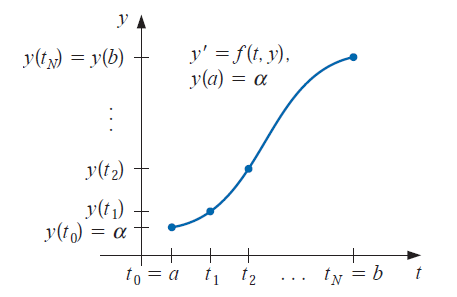
\includegraphics[width=0.65\textwidth]{Euler1.png}
\caption{}
\label{tab:fig9}
\end{figure*} 

\begin{multicols}{2}
\begin{figure}[H]
\centering
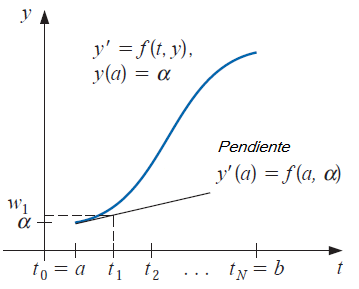
\includegraphics [ width =0.5\textwidth ]{Euler2.png}
\caption{}
\label{tab:fig10}
\end{figure}
\begin{figure}[H]
\centering
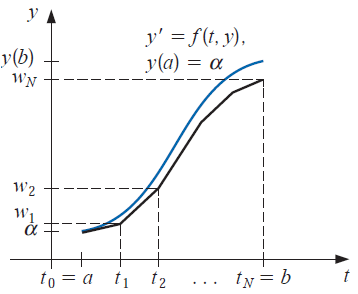
\includegraphics [ width =0.5\textwidth ]{Euler3.png}
\caption{}
\label{tab:fig11}
\end{figure}
\end{multicols}

\subsection*{4.2 Método de Euler mejorado}

Dado que el objeto de las técnicas numéricas es determinar aproximaciones precisas con el mínimo esfuerzo, necesitamos una medida para comparar la eficiencia de varios métodos de aproximación. La primera de ellas que consideramos se denomina \textbf{error de truncamiento local}.

Considere el problema del valor inicial

\begin{equation*}
    y'=f(t,y), \ \  a\leq t\leq b, \ \ y(a)=\alpha, 
\end{equation*}

el método diferencial

\begin{equation*}
\begin{split}
    w_0&=\alpha \\
    w_{i+1}&=w_i+h\Phi(t_i,w_i), \ \ para \ cada \ i=0,1,2, \dotsc, N-1.
\end{split}
\end{equation*}

tiene el \textbf{error de truncamiento local}

\begin{equation*}
    \tau_{i+1}(h)=\frac{y_{i+1}-(y_i+h\Phi(t_i,y_i))}{h}=\frac{y_{i+1}-y_i}{h}-\Phi(t_i,y_i).
\end{equation*}

para cada $i=0,1,2, \dotsc, N-1$ donde $y_i$ y $y_{i+1}$ denotan la solución al tiempo $t_i$ y $t_{i+1}$ respectivamente.
\\

En afán de ir reduciendo cada vez más el error relacionado al método se busca optimizar el proceso de aproximación, ahora bien, para desarrollar un método más preciso que el de Euler se puede modificar éste para mejorarlo, de esta manera surge el \textbf{método de Euler modificado} el cual consta en realizar una corrección intermedia a cada iteración, primero se estima el punto sucesivo y enseguida se hace la corrección de la forma:

\begin{equation*}
    w_{i+1}=w_i+\frac{h}{2}(f(t_i,w_i)+f(t_i+h,w_i+hf(t_i,w_i))).
\end{equation*}

Entonces el algoritmo resultante es:

\begin{equation*}
\begin{split}
    w_0&=\alpha \\
    w^*_{i+1}&=w_i+hf(t_i,w_i), \ \ Estimacion \\
    w_{i+1}&=w_i+\frac{h}{2}(f(t_i,w_i)+f(t_i+h,w^*_{i+1})) \ \ Correccion \\ 
    & \ \ \ \ \ para \ cada \ i=0,1,2, \dotsc, N-1.
\end{split}
\end{equation*}

Y, por lo tanto, el código es el siguiente:


\begin{tcolorbox}[colback=blue!15!]
\subsubsection*{Método de Euler modificado}
Para aproximar la solución del problema con valores iniciales

\begin{equation*}
    y'=f(t,y), \ \  a\leq t\leq b, \ \ y(a)=\alpha,
\end{equation*}

en un intervalo [a,b] dividido en (N+1) del mismo tamaño:
\\ \\
ENTRADA Puntos extremos a,b; entero N; condición inicial $\alpha$.

SALIDA Aproximación $w$ a $y$ en $(N+1)$ valores de $t$.
\\ \\
PASO 1 Asigna h=(b-a)/N;

\ \ \ \ \ \ \ \ t=a;

\ \ \ \ \ \ \ \ $w=\alpha$;

\ \ \ \ \  SALIDA (t,w).

PASO 2 Para $i=1,2,\dotsc, N$ ejecuta los pasos 3 y 5.

\ \ \ \  PASO 3 Asigna $w^*=w+hf(t,w)$; (Estima $w_i$.)

\ \ \ \  PASO 4 Asigna $w=w+\frac{1}{2}h(f(t,w)+f(t+h,w^*))$; (Corrige $w_i$.)

\ \ \ \ \ \ \ \ \ \ \ \ \ \ \ \ \ \ \ \ \ \ \ \ \ \ \ \ \ $t=a+ih$; (calcula $t_i$.)

\ \ \ \  PASO 5  SALIDA (t,w)

PASO 6 Alto.

\end{tcolorbox}

\subsection*{4.3 Método de Runge-Kutta}

Los métodos de Runge-Kutta tienen el error de truncamiento local de alto orden de los métodos de Taylor, pero eliminan la necesidad de calcular y evaluar las derivadas de $f(t, y)$. Antes de presentar las ideas detrás de su derivación, debemos considerar el Teorema de Taylor en dos variables.

\subsubsection*{Teorema de Taylor en dos variables}
Supongamos que $f(t, y)$ y todas sus derivadas parciales de orden menor o igual a $n+1$ son continuas en $D = \{ (t, y) | a\leq t \leq b, c \leq y \leq d \}$, y sea $(t_0, y_0) \in D$. Para todo $(t, y) \in D$, existe $\xi$ entre $t$ y $t_0$ y $\mu$ entre $y$ e $y_0$ con

\begin{equation*}
    f(t,y)=P_n(t,y)+R_n(t,y),
\end{equation*}

donde

\begin{equation*}
\begin{split}
    P_n(t,y)=&f(t_0,y_0)+ \left[ (t-t_0)\frac{\partial f}{\partial t} (t_0,y_0) + (y-y_0)\frac{\partial f}{\partial t} (t_0,y_0) \right] \\ 
    & + \left[ \frac{(t-t_0)^2}{2}\frac{\partial^2 f}{\partial t^2} (t_0,y_0) + (t-t_0)(y-y_0)\frac{\partial^2 f}{\partial t \partial y} (t_0,y_0) + \frac{(y-y_0)^2}{2}\frac{\partial^2 f}{\partial y^2}(t_0,y_0) \right] \\
    & + \dotsi + \left[ \frac{1}{n!} \sum_{j=0}^n \binom{n}{j}(t-t_0)^{n-j}(y-y_0)^j \frac{\partial^n f}{\partial t^{n-j} \partial y^j}(t_0,y_0) \right].
\end{split}
\end{equation*}

Y

\begin{equation*}
    R_n(t,y)=\frac{1}{(n+1)!} \sum_{j=0}^{n+1} \binom{n+1}{j}(t-t_0)^{n+1-j}(y-y_0)^j \frac{\partial^{n+1}f}{\partial t^{n+1-j} \partial y^j}(\xi,\mu).
\end{equation*}

La función $P_n(t, y)$ se llama enésimo polinomio de Taylor en dos variables para la función $f$ sobre $(t_0, y_0)$, y $R_n(t, y)$ es el término restante asociado con $P_n(t, y)$.

\subsubsection*{Método de Runge-Kutta de orden dos}

El primer paso para derivar un método de Runge-Kutta es determinar los valores para $a_1$, $\alpha_1$ y $\beta_1$ con la propiedad de que $a_1 f(t+\alpha_1,y+\beta_1)$ se aproxima:

\begin{equation*}
    T^{(2)}(t,y)=f(t,y)+\frac{h}{2}f'(t,y),
\end{equation*}

con un error no mayor que $O(h^2)$, que es igual al orden del error de truncamiento local para el método de Taylor de orden dos. Ya que

\begin{equation*}
    f'(t,y)=\frac{df}{dt}(t,y)=\frac{\partial f}{\partial t} (t,y) + \frac{\partial f}{\partial y} (t,y)\cdot y'(t) \ \ , \ \ y'(t)= f(t,y)
\end{equation*}

entonces:

\begin{equation*}
    T^{(2)}(t,y)=f(t,y)+\frac{1}{2}\frac{\partial f}{\partial t} (t,y) + \frac{1}{2}\frac{\partial f}{\partial y} (t,y)\cdot f(t,y).
\end{equation*}

Expandiendo 

\begin{equation*}
\begin{split}
       a_1 f(t+\alpha _1, y + \beta _1)=&a_1f(t,y)+a_1\alpha _1 \frac{\partial f}{\partial t} (t,y) + a_1 \beta _1 \frac{\partial f}{\partial y} (t,y) \\
       & + a_1 \cdot R_1(t+\alpha _1, y + \beta _1).
\end{split}
\end{equation*}

Donde

\begin{equation*}
    R_1(t+\alpha _1, y + \beta _1) = \frac{\alpha_1^2}{2} \frac{\partial^2 f}{\partial t^2} (\xi,\mu) + \alpha _1\beta _1 \frac{\partial^2 f}{\partial t \partial y} (\xi,\mu) + \frac{\beta_1^2}{2} \frac{\partial^2 f}{\partial y^2} (\xi,\mu)
\end{equation*}

para algún $/xi$ entre $t$ y $t+\alpha_1$ y $\mu$ entre $ y + \beta _1$.
\\
Igualando los coeficientes de $f$ y sus derivadas se obtiene:

\begin{equation*}
    f(t,y): a_1=1; \ \ \ \ \frac{\partial f}{\partial t} (t,y):a_1 \alpha_1=\frac{h}{2}; \ \ \ \ \frac{\partial f}{\partial y} (t,y):a_1 \beta_1=\frac{h}{2}f(t,y).
\end{equation*}

Por lo tanto los parámetros $a_1$, $\alpha_1$ y $\beta_1$ son:

\begin{equation*}
    a_1=1; \ \ \ \ \alpha_1=\frac{h}{2}; \ \ \ \ \  \beta_1=\frac{h}{2}f(t,y).
\end{equation*}

Entonces

\begin{equation*}
    T^{(2)}(t,y)=f \left(t+ \frac{h}{2},y+\frac{h}{2}f(t,y)\right)-R_1 \left(t+ \frac{h}{2},y+\frac{h}{2}f(t,y)\right)
\end{equation*}

PP 285